\documentclass[a4paper]{ctexart}
\usepackage{xeCJK}
\usepackage{setspace}
\usepackage{graphicx,wrapfig}
\usepackage{fontspec,xunicode,xltxtra}
\usepackage{fancyhdr,titlesec,titletoc}
\usepackage[titletoc]{appendix}
\usepackage[top=29mm,bottom=29mm,left=31.8mm,right=31.8mm]{geometry}
\usepackage{enumerate,enumitem}
\usepackage{caption,subcaption}
\usepackage{amsmath,amssymb,bm,array}
\usepackage{cite}
\usepackage{diagbox}
\usepackage{algorithm,algorithmicx,algpseudocode}
\usepackage{multirow}
\usepackage[super]{gbt7714}
\setmainfont{Times New Roman}
\setCJKmainfont[BoldFont={Songti SC Bold}]{SimSun}
\setCJKfamilyfont{heiti}{SimHei}
\renewcommand{\heiti}{\CJKfamily{heiti}\fontspec{Times New Roman}}
\renewcommand{\appendixpagename}{附录}

\usepackage{listings}
\usepackage[usenames,dvipsnames]{color}
\definecolor{MyDarkGreen}{rgb}{0.0,0.4,0.0}
\lstloadlanguages{Matlab}
\lstset{language=Matlab,
        frame=single,
        basicstyle=\small\ttfamily,
        keywordstyle=[1]\color{Blue}\bfseries,
        keywordstyle=[2]\color{Purple},
        keywordstyle=[3]\color{Blue}\underbar,
        identifierstyle=,
        commentstyle=\usefont{T1}{pcr}{m}{sl}\color{MyDarkGreen}\small,
        stringstyle=\color{Purple},
        showstringspaces=false,
        tabsize=5,
        morekeywords={xlim,ylim,var,alpha,factorial,poissrnd,normpdf,normcdf},
        morekeywords=[2]{on, off, interp},
        morekeywords=[3]{FindESS, homework_example},
        morecomment=[l][\color{Blue}]{...},
        numbers=left,
        firstnumber=1,
        numberstyle=\tiny\color{Blue},
        stepnumber=5
        }
\newcommand{\matlabscript}[2]
  {\begin{itemize}\item[]\lstinputlisting[caption=#2,label=#1]{#1.m}\end{itemize}}

\newcommand{\mycaptionfont}{\heiti\zihao{5}}
\captionsetup[figure]{name={\mycaptionfont 图},labelsep=period}
\captionsetup[table]{name={\mycaptionfont 表},labelsep=period}
\floatname{algorithm}{\mycaptionfont 算法}
\captionsetup[algorithm]{labelsep=period}
\renewcommand{\captionfont}{\mycaptionfont}
\renewcommand{\captionlabelfont}{\mycaptionfont}

\ctexset {
	section = {
		number = \arabic{section},
		format = \zihao{4}\bfseries,
	},
	subsection = {
		number = \arabic{section}.\arabic{subsection},
		format = \zihao{-4}\bfseries,
	},
	subsubsection = {
		number = \arabic{section}.\arabic{subsection}.\arabic{subsubsection},
		format = \zihao{-4}\bfseries,
	}
}
\setlist[enumerate]{itemindent=2em,listparindent=2em,leftmargin=0em,label=\arabic*、}

\setlength\parskip{.5\baselineskip}
\fancypagestyle{plain}{\pagestyle{fancy}}%改变章节首页页眉
\pagestyle{fancy}
\lhead{\kaishu~RFID无线射频识别实验报告~}
\rhead{\kaishu~1030616134~尹达恒}
\cfoot{\thepage}

\begin{document}

\begin{center}
	{\zihao{-3}\textbf{实验四\quad Matlab仿真实现安全认证协议}}

	{\zihao{-4}尹达恒}\\[-1mm]

	{\zihao{5}(江南大学物联网工程学院,江苏\quad 无锡)}
\end{center}

\renewcommand{\baselinestretch}{1.3}
\zihao{-4}
\section{实验目的}
通过本次实验,了解基于哈希函数的认证协议,将理论知识与实际相结合。

\section{实验设备}
MATLAB编程软件

\section{实验原理}\label{实验原理}
\subsection{哈希函数}
定义:将任意长度的输入x映射为定长为n的输出y。
哈希函数在密码应用中的主要作用是提供数据完整性和消息验证。因此,需满足单边质询条件:
\begin{itemize}
	\item 从输出y并不能计算出输入x的值;
	\item 同时对输入x而言,不存在两个不同的输入值x,x1(x≠x1)满足Hash(x)=Hash(x1)。
\end{itemize}
\subsection{哈希锁方案}
哈希锁方案是标签不用存储存取关键字,只需存储该关键字的哈希值,如图1所示。标签只存储一个低耗的哈希函数h,一个唯一的标识ID和密钥k的哈希值Hash\_k=Hash(k)。后台服务器存储每个标签的密钥k和Hash\_k。
\begin{itemize}
	\item 质询:读写器向标签发送请求;
	\item 响应:标签返回Hash\_k到读写器;
	\item 验证:读写器将接收到的Hash\_k传递给数据库,查找与之对应的密钥k,并与存储的Hash\_k进行比较。如果这两个值匹配,标签就将自己的ID发送给读写器。
\end{itemize}
\begin{figure}[htbp]
	\centering
	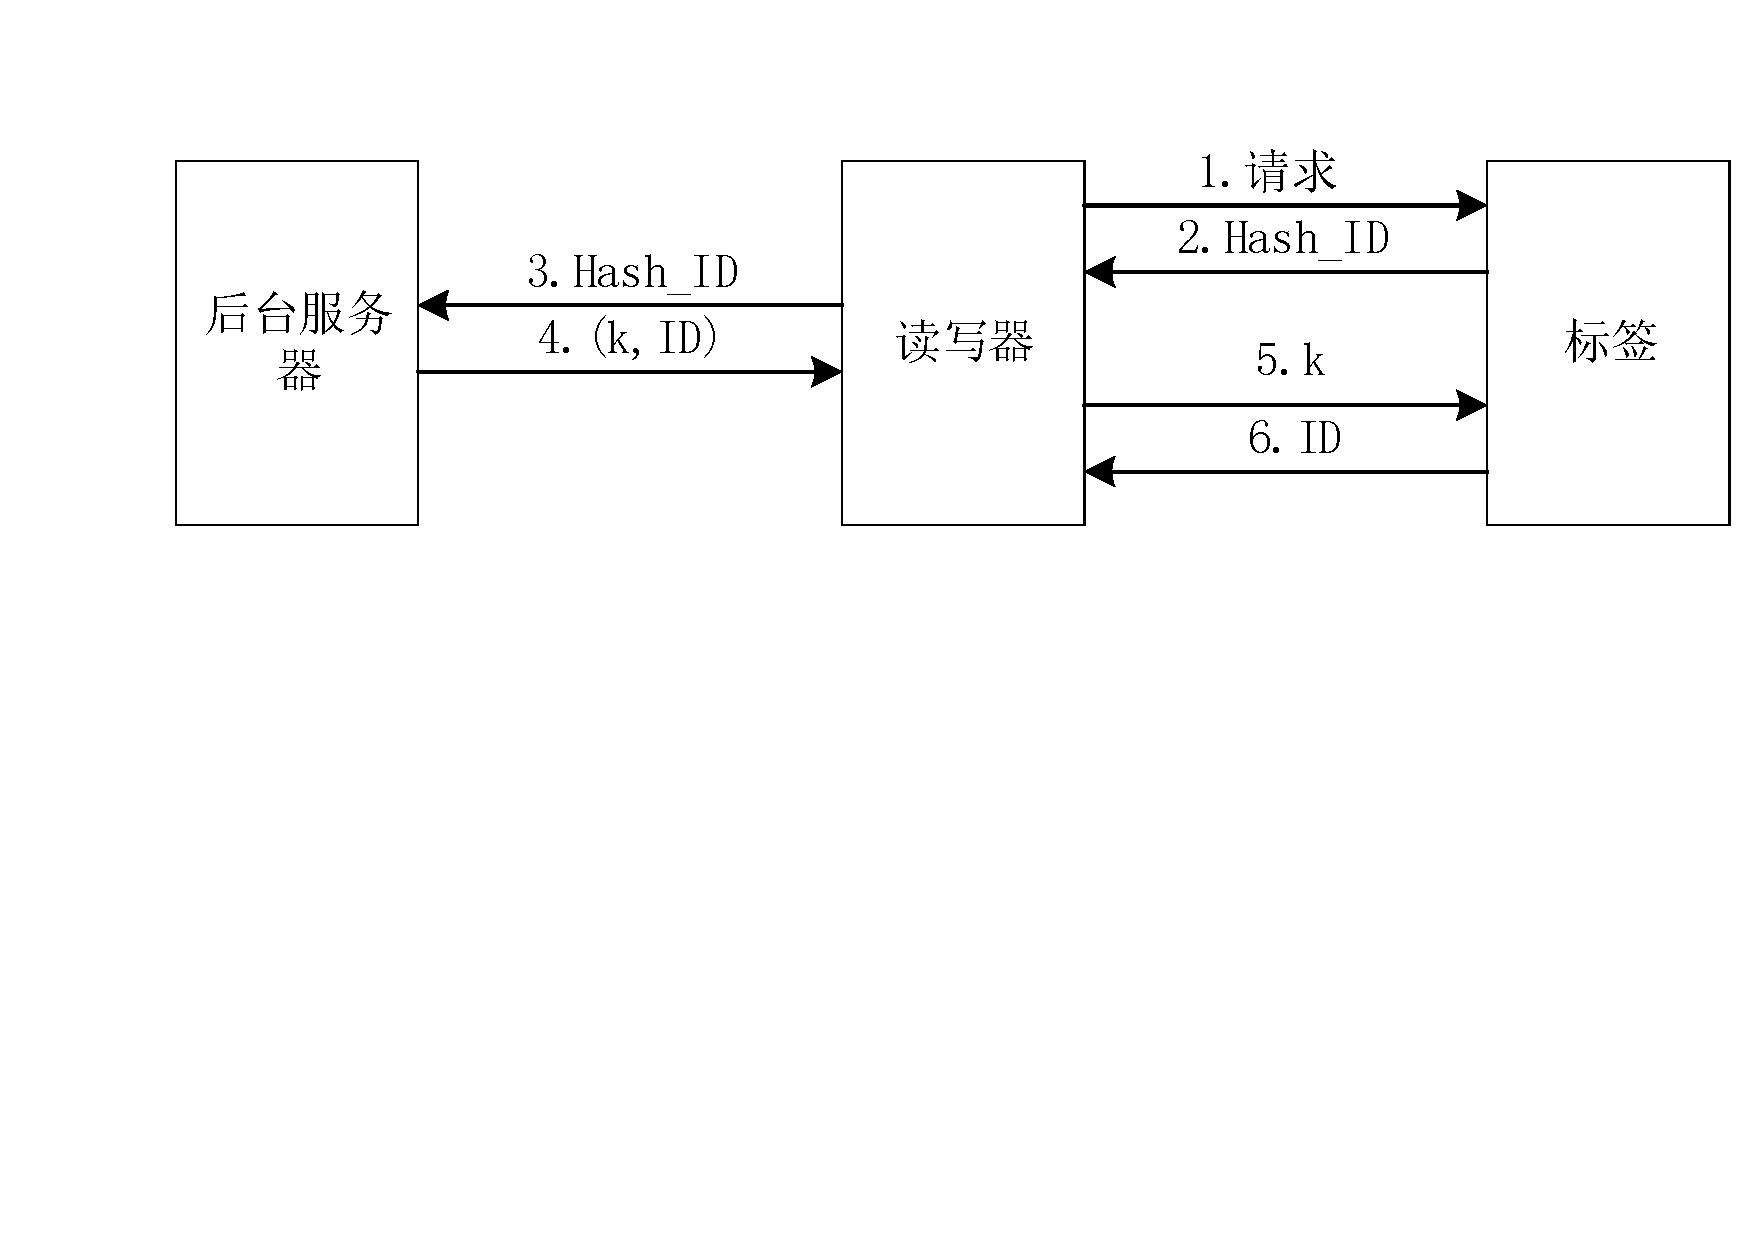
\includegraphics[width=0.8\textwidth]{figure/1.pdf}
	\caption{哈希锁方案}
\end{figure}

\section{实验步骤}
\subsection{设计思路}
定义三个子函数,即读写器、标签、后台服务器,设计每个部分的内部函数,设计一个基于哈希函数的认证协议。

哈希锁方案是最基本的认证方案,但也存在着不足,即Hash\_k是不变的,攻击者可以通过窃听来识别每个标签,并追踪该标签从而确定标签持有者的位置隐私。因此,可在哈希锁方案的基础上,设计其他改进协议,如随机哈希锁方案、哈希链方案、双向认证协议等,并得到所需要的设计结果:
\begin{itemize}
	\item 运行成功的图形结果;
	\item 所设计协议的运行时间。
\end{itemize}

\subsection{程序结构}
\begin{enumerate}[label=\arabic*、]
	\item 后台服务器:classdef Server
	      该类在初始化时接受一个字符串数组和加密方法,以此生成密钥哈希值数据库。该类包含两个方法:
	      \begin{itemize}
		      \item Verify:输入一个hash\_k,在数据库中查找对应的k和ID并返回,如果查不到则报错;
		      \item getTags:返回数据库中所有hash\_k和对应标签ID。
	      \end{itemize}
	\item 标签:classdef Tag
	      该类在初始化时接受一个ID、一个hash\_k和加密方法。该类包含两个方法:
	      \begin{itemize}
		      \item Request:返回hash\_k值;
		      \item Verify:输入密钥进行哈希验证,如验证成功则返回ID值
	      \end{itemize}
	\item 读写器主程序:
	      \begin{itemize}
		      \item 初始化:主程序初始化时将生成一个随机的密钥字符串数组,将其输入到Server类中生成数据库,并调用getTags方法生成标签信息;随后标签信息将用于生成一个标签数组。
		      \item 向标签发送请求:调用标签类的Request方法获取标签hash\_k进行比较。如果这两个值匹配,标签就将自己的ID发送给读写器。
		      \item 服务器端验证:调用服务器类的Verify方法,输入上一步中的hash\_k进行验证,获取密钥k和ID。
		      \item 标签验证:调用标签类的Verify方法,输入密钥k进行验证,获取标签ID。
		      \item 读写器验证:比对标签发来的ID和服务器端获取到的标签ID,如相等则验证通过。
	      \end{itemize}
\end{enumerate}


\section{实验结果}
\subsection{哈希锁方案程序输出}
\begin{lstlisting}
初始化数据库:
ID=1,k=AGqvyYLAK,hask_k=9b02ef25b1ff6b1729e75848db73bd68
ID=2,k=ArMPy5m5g,hask_k=5c0d69e4ac80fc6dbcacb7b494ff7243
ID=3,k=AZgsmFzxz,hask_k=111f37c3d042157f94c6a8fd64a9a871
ID=4,k=AXPQSl0R5,hask_k=572afbd5299c56bd32e513aed96f1b4e
标签初始化:ID=1,hash_k=9b02ef25b1ff6b1729e75848db73bd68
标签初始化:ID=2,hash_k=5c0d69e4ac80fc6dbcacb7b494ff7243
标签初始化:ID=3,hash_k=111f37c3d042157f94c6a8fd64a9a871
标签初始化:ID=4,hash_k=572afbd5299c56bd32e513aed96f1b4e
标签收到请求,发回hash_k=9b02ef25b1ff6b1729e75848db73bd68
服务器验证成功:ID=1,k=AGqvyYLAK
标签验证成功,k=AGqvyYLAK,hash_k=9b02ef25b1ff6b1729e75848db73bd68
时间已过 0.010616 秒。
标签收到请求,发回hash_k=5c0d69e4ac80fc6dbcacb7b494ff7243
服务器验证成功:ID=2,k=ArMPy5m5g
标签验证成功,k=ArMPy5m5g,hash_k=5c0d69e4ac80fc6dbcacb7b494ff7243
时间已过 0.002059 秒。
标签收到请求,发回hash_k=111f37c3d042157f94c6a8fd64a9a871
服务器验证成功:ID=3,k=AZgsmFzxz
标签验证成功,k=AZgsmFzxz,hash_k=111f37c3d042157f94c6a8fd64a9a871
时间已过 0.001541 秒。
标签收到请求,发回hash_k=572afbd5299c56bd32e513aed96f1b4e
服务器验证成功:ID=4,k=AXPQSl0R5
标签验证成功,k=AXPQSl0R5,hash_k=572afbd5299c56bd32e513aed96f1b4e
时间已过 0.001550 秒。
\end{lstlisting}

\newpage
\appendix
\appendixpage
\section{服务器类}
\begin{lstlisting}
classdef Server
    properties(Access=private)
        database;
        key_length;
    end
    
    methods(Access=public)
        function obj = Server (keys,meth)
            fprintf('初始化数据库:\n');
            obj.database={};
            n=size(keys);
            for i=1:(n(1))
                obj.database.(keys(i,:))=hash(keys(i,:),meth);
                fprintf('ID=%d,k=%s,hask_k=%s\n',i,
                        keys(i,:),obj.database.(keys(i,:)));
            end
            obj.key_length=length(obj.database.(keys(i,:)));
        end
        function [key,ID] = Verify(obj,hash_k)
            keys=fieldnames(obj.database);
            for ID=1:length(keys)
                key=keys{ID,1};
                if strcmp(obj.database.(key),hash_k)
                    fprintf('服务器验证成功:');
                    fprintf('ID=%d,k=%s\n',ID,key);
                    return;
                end
            end
            fprintf('hash_k=%s 服务器验证不成功',hash_k);
            ID=0;
        end
        function tags = getTags(obj)
            keys=fieldnames(obj.database);
            tags=repmat(' ',length(keys),obj.key_length);
            for ID=1:length(keys)
                key=keys{ID,1};
                tags(ID,:)=obj.database.(key);
            end
        end
    end
end
\end{lstlisting}
\section{标签类}
\begin{lstlisting}
classdef Tag
    properties
        ID;
        hash_k;
        meth;
    end
    
    methods
        function obj = Tag(ID,hash_k,meth)
            obj.ID=ID;
            obj.hash_k=hash_k;
            obj.meth=meth;
            if ID~=0
                fprintf('标签初始化:ID=%d,hash_k=%s\n',ID,hash_k);
            end
        end
        
        function hash_k = Request(obj)
            hash_k=obj.hash_k;
            fprintf('标签收到请求,发回hash_k=%s\n',hash_k);
        end
        
        function ID = Verify(obj,key)
            ID=0;
            if strcmp(hash(key,obj.meth),obj.hash_k)
                ID=obj.ID;
                fprintf('标签验证成功,k=%s,hash_k=%s\n',key,obj.hash_k);
            end
        end
    end
end
\end{lstlisting}
\section{读写器主程序}
\begin{lstlisting}
clear;
N=4;
meta='abcdefghijklmnopqrstuvwxyzABCDEFGHIJKLMNOPQRSTUVWXYZ0123456789';
keys=[repmat('A',N,1),meta(randi([1,length(meta)],N,8))];
server=Server(keys,'MD5');
hash_ks=server.getTags();
n=size(hash_ks);
tags=[Tag(0,'','')];
for ID=1:n(1)
    tags(ID)=Tag(ID,hash_ks(ID,:),'MD5');
end

for ID=1:n(1)
    tic
    tag=tags(ID);
    hash_k=tag.Request();
    [k,IDs]=server.Verify(hash_k);
    IDt=tag.Verify(k);
    if strcmp(IDs,IDt)
        fprintf('标签%d验证成功',ID);
    end
    toc
end
\end{lstlisting}
\end{document}